\paragraph{Piecewise Polynomials}
\tB{It involves fitting separate low-degree polynomials over different 
regions of $X$.}\\
The points where the coefficients change are called \tR{\emph{knots}}.
It is a function $f(X)$ that is obtained by dividing the domain of $X$ into contiguous intervals,
and representing $f$ by a separate polynomial in each interval.
More generally, an order$-M$ spline with knots $\zeta_{j}, j\in\inter{1}{K}$ is a 
piecewise-polynomial of order $M$, and has continuous derivatives up to order $M-2$.
Likewise the general form for the truncated-power basis set would be:
\begin{align*}
h_{j}(X) &= X^{j-1}, &j\in\inter{1}{M}\\
h_{M+j} &=\left(X-\zeta_{l}\right)_{+}^{M-1}, &l\in\inter{1}{K}
\end{align*}

%\paragraph{Constraints and Splines}
%We can fit a piecewise polynomial under the constraint that the fitted
%curve must be continuous.

\paragraph{The spline Basis Representation}
A cubic spline with $K$ knots can be modeled as:
\begin{center}
\enc{$
y_{i}=\beta_{0}+\su{{r=1}}{K+3}\beta_{r}b_{r}(x_{i})
$}
\end{center}
for an appropriate choice of \emph{basis functions} $\prth{b}{i}{K+3}$\\
The most direct way to represent cubic spline is \tB{to start off with
a basis for a cubic polynomial -namely, $x, x^{2}, x^{3}$ -and then add
one \emph{truncated power basis} function per knot}.
A truncated power basis function, for a cubic polynomial, is defined as:
\begin{center}
\enc{$
h(x,\zeta) = (x-\zeta)_{+}^{3}=
\left\{
\begin{array}{ll}
	(x-\zeta)^{3}&\mbox{if }x>\zeta\\
	0&\mbox{otherwise}
\end{array}
\right.
$}
\end{center}
where $\zeta$ is the knot.\\
In order to fit a cubic spline to a data set with $K$ knots, we perform
least squares regression with an intercept and $3+K$ predictors of the
form $X, X^{2}, X^{3}, h\left(X,\zeta_{1}\right), h\left(X,\zeta_{2}\right),,..,h\left(X,\zeta_{K}\right)$ where $\prth{\zeta}{i}{K}$ are the
knots. This amounts to estimating a total of $K+4$ regression 
coefficients.\\
Cubic splines are popular because most human eyes cannot detect 
discontinuity at the knots.

\begin{figure}[H]
	\begin{center}
		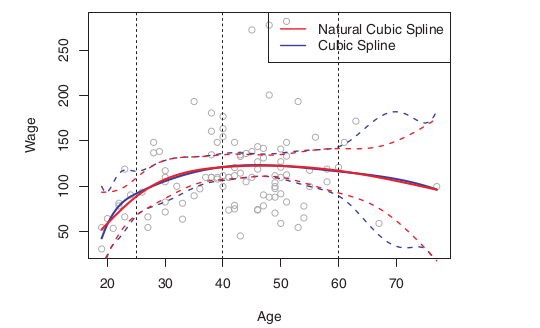
\includegraphics[width=.7\textwidth]{./chap/1chap/6sec/images/1splines.png}
	\end{center}
	\caption{A cubic spline and a natural cubic spline, with 3 
	knots, fit to a subset of the Wage data, confidence interval as
	dashed lines.}
	\label{fig:6.1splines}
\end{figure}
A natural spline is a regression spline with additional boundary 
constraints: the function is required to be linear at the boundary (in
the region where $X$ is smaller than the smallest knot, or larger than
the largest knot).\\
\tB{This frees up $4$ degrees of freedom ($2$ constraints each in both boundary regions), which
can be spent more profitably by sprinkling more knots in the interior region. }
A natural cubic spline with $K$ knots is represented by $K$ basis functions.
\begin{center}
	$\begin{cases}
		N_{1}(X) = 1\\
		N_{2}(X) = X
	\end{cases}
	,~ N_{k+2}(X) = d_{k}(X)-d_{K-1}(X)$
\end{center}
where $d_{k}(X) = \dfrac{\left(X-\zeta_{k}\right)_{+}^{3} - \left(X-\zeta_{K}\right)_{+}^{3}}{
\zeta_{K}-\zeta_{k}}$

\paragraph{Choosing the Number and Locations of the Knots}
One option is \tB{to place more knots in places where we feel the 
function might vary most rapidly}, and to place fewer knots where it 
seems more stable.\\
\sR{For the number of knots we can use cross-validation.}

\begin{python}
import pandas 
import statsmodels.api as sm
import sklearn
from sklearn.model_selection import KFold
import patsy
from patsy import dmatrix

# Choosing the good number of knots
y, x = df.iloc[:, 0], df.iloc[:, 1]
kf = KFold(n_splits=5)
n = 52
cv_set = {str(i):0 for i in range(1, n)}
for i in range(1, n):
    n_knots = i
    knot_list = np.quantile(x, np.linspace(0, 1, n_knots + 2))[1:-1]
    mse_list = []
    for train, test in kf.split(x):
        x_natural = dmatrix('cr(x, knots=knot_list)', {'x':x[train]})
        fit_natural = sm.GLM(y[train], x_natural).fit()
        yhat = fit_natural.predict(dmatrix('cr(x, knots=knot_list)', {'x':x[test]}))
        mse = ((yhat-y[test])**2).mean()
        # mse_list.append(mse)
        mse_list.append(mse)
        # print(mse)
    cv_set[str(i)] = np.array(mse_list).mean()
cv_list = list({k:v for k,v in sorted(cv_set.items(), key=lambda item: item[1])})


n_knots = int(cv_list[0])
knot_list = np.quantile(x, np.linspace(0, 1, n_knots + 2))[1:-1]
# Natural
x_natural = dmatrix('cr(x, knots = knot_list)', {'x':x})
fit_natural = sm.GLM(y, x_natural).fit()

# Create spline
xp = np.linspace(x.min(), x.max(), 50)
line_natural = fit_natural.predict(dmatrix('cr(xp,knots=knot_list)',
                                           {'xp':xp}))

plt.figure()
plt.scatter(df.iloc[:, 0], df.iloc[:, 1])
plt.plot(xp, line_natural, color='red', label="Natural Spline Regression")
for k in knot_list:
    plt.axvline(k, color='gray', ls='--')
plt.legend()
plt.show()
\end{python}
\paragraph{Comparison to Polynomial Regression}
Regression splines give superior results to polynomial regression.\\
\sB{This is because unlike polynomials, which must use a higher degree 
to produce flexible fits, splines introduce flexibility by increasing
the number of knots but keeping the degree fixed.}\\
Splines produce also more stable estimates.
